
\section{Introduction}

% Supertree estimation is the problem of computing a tree on a set $S$ of taxa from a set of estimated  trees (called ``source trees") on subsets of $S$. 
% Traditionally, the purpose of supertree estimation was 
% to combine published species trees estimated by different research groups around the world, using different datasets and different methods. 
% Supertree methods have been used
% to construct many species trees,
% %\cite{placental,marsupial,cpl,THPL,supertrees-placental,seabirds,supertree-sanderson,pisani2007supertrees},
% and the development of supertree methods is an area 
% of very active research
% (see 
% \cite{bininda2004phylogenetic} for some of the early literature,
% and \cite{mrl,superfine,Akanni-MLsupertree} for some more recent methods).

% More recently, supertree estimation has been used within divide-and-conquer frameworks, in which a large and potentially heterogeneous dataset is divided into overlapping smaller subsets, trees are estimated on each subset, and then combined into a tree on the full dataset using a supertree method. 
% These divide-and-conquer methods thus enable the application of  statistical phylogeny estimation methods to scale to larger datasets
% \cite{dactal,BayzidRECOMBCG2014,afc,dcm1-huson}.
% Each of these methods has been able to improve the accuracy and/or speed of its base method.  
% Thus, supertree computation provides an essential tool for both moderate- and large-scale phylogeny estimation, and is relevant to both gene tree estimation and species tree estimation. 

One of the popular approaches to supertree estimation is the
NP-hard
Robinson-Foulds Supertree problem \cite{bansal2010robinson}, which 
seeks a binary tree that has the minimum total Robinson-Foulds
\cite{RF} distance to the input source trees.
The best known local search 
heuristic for the Robinson-Foulds Supertree
is MulRF \cite{mulrf}, but
PluMiST \cite{plumist} is a new method that
shows promise; 
to our knowledge, there are no
other methods that are competitive with these two.

One of the exciting properties of the
Robinson-Foulds Supertree problem is that it is closely
related to  the Maximum Likelihood Supertree problem,
which seeks a supertree that is the most likely to
have produced the observed source trees under a simple
exponential
model of phylogenetic error \cite{ml-supertree}.
Although the two problems are not identical
(as established in \cite{BryantSteel2009}),
it seems likely that 
good solutions to the
Robinson-Foulds Supertree problem will 
be good solutions to the Maximum 
Likelihood Supertree problem. 
However, 
the only technique for
the Maximum Likelihood Supertree problem that we are
aware of,  L.U.-st \cite{Akanni-MLsupertree},
is very computationally intensive, making it
infeasible for use
on biological datasets \cite{Akanni-Bayesian}.

In this paper, we report 
on a new method, FastRFS (Fast Robinson-Foulds Supertrees) for 
finding optimal Robinson-Foulds Supertrees in a constrained search space.
Unlike the previous methods for Robinson-Foulds Supertrees, which depended on heuristic searches through 
tree space, the method we have designed uses dynamic programming (DP) to 
find an exact solution to the Robinson-Foulds Supertree 
problem within a constrained search space. 

This algorithmic strategy
of using dynamic programming to find
a species tree optimizing some criterion within
a constrained search space
was first used
in 
\cite{hallett2000new};
since that time, the approach has been used in 
other phylogenetic estimation methods
\cite{bryant2001constructing,MDC,yu2011algorithms,bayzid2013inferring,ASTRAL,ASTRAL2}.
Most of these methods constrain the search
space for their
optimization problem by computing a set $X$ of allowed bipartitions
(i.e., splits of the leafset into two parts, each defined by
deleting edges in the species tree that will be constructed)
from the input, and require that the output tree 
draw its bipartitions from $X$.
These methods run in time that is polynomial in the 
number of species, source trees, and $|X|$.
Many of these methods
specify
$X$ to be  the set of bipartitions
in the input source trees, but expanding 
the set
can improve accuracy \cite{ASTRAL2}.


The supertree method we present, FastRFS,
is a combination
of the polynomial time dynamic programming algorithm for
the constrained Robinson-Foulds Supertree problem
we have developed and the technique we use
to define the set $X$ from the input source trees.
The basic FastRFS method uses  
ASTRAL-2
to define the set $X$ of allowed bipartitions
from the input set of source trees.
We also explore an enhanced version where we add additional
 bipartitions (beyond those computed by ASTRAL-2)
to the set X defined by ASTRAL-2. We define the additional
bipartitions by computing fast supertrees on the input
set, and then add their bipartitions to $X$;
this
 approach ensures that we find
RFS criterion scores that are at least as good as the trees we use
to define the set $X$ of allowed
bipartitions,
and also at least as good as the trees obtained by the 
basic
FastRFS method.
By only adding bipartitions from supertrees that we 
can compute quickly, the enhanced FastRFS method is able to complete
quickly, and provides improved criterion scores.

We evaluate these two versions of FastRFS in comparison to 
leading methods for supertree estimation
on a collection of biological and simulated datasets
 with 100 to 2228 species
that were used in prior publications to evaluate supertree methods
\cite{smidgen,superfine,mrl}.
We compare FastRFS to 
PluMiST, the current best performing method
(in terms of criterion scores)
 for the Robinson-Foulds Supertree problem,
and also to
MulRF, the most well known software for this optimization problem.
We also compare FastRFS to 
 Matrix Representation with Likelihood (MRL) \cite{mrl},  
 ASTRID \cite{ASTRID}, and  ASTRAL-2 \cite{ASTRAL2}.
MRL is the maximum likelihood counterpart
to the well known Matrix Representation with Parsimony (MRP) method, and
has produced topologically more accurate supertrees than 
leading MRP heuristics \cite{mrl}. ASTRID and ASTRAL-2 are
methods for species tree estimation that  take 
gene tree heterogeneity arising from incomplete lineage sorting into account,
and have had good accuracy on large phylogenomic datasets.
We evaluate these methods with respect to
RFS criterion scores (which can
be evaluated on both simulated and biological datasets), 
topological accuracy in estimating the true supertree (which
can only be evaluated on simulated datasets), and wall clock running time.




\section{Materials and Methods}



Every model tree and estimated supertree in this study is a 
fully resolved tree,
and no two leaves have the same label; the source
trees are unrooted trees with leaves drawn from 
(possibly proper)
subsets of the full set of taxa, and may contain
polytomies (nodes of degree greater than three).
We let $T|Q$ denote the tree obtained by restricting the tree $T$ to the subset $Q$ of its leafset, and then suppressing nodes of degree two. 
% We let $\mathcal{L}(T)$ denote the leafset of a tree $T$. 
% The deletion of an edge $e$ from a tree $T$ induces a 
% bipartition of $\mathcal{L}(T)$ into two sets $A$ and $B$,
% denoted by $[A,B]$. Every unrooted 
% tree $T$ is defined by its set $Bip(T)$ of bipartitions. 
% The Robinson-Foulds (RF) distance between trees $T$ and $T'$ that are on the same leafset is the number of bipartitions that are in one tree but not the other (i.e., $RF(T,T') = |Bip(T) \triangle Bip(T')|$). Note that when $T$ and $T'$ have the same leafset, then $RF(T,T')=0$ if and only if $T=T'$.

We extend the
definition of RF distance to trees $t$ and $T$ with
nested leafsets (i.e., $\mathcal{L}(t) \subseteq  \mathcal{L}(T)$)
to be the RF distance between $T|\mathcal{L}(t)$ and $t$, and denote this distance by $RF(T,t)$.
Given a set $\mathcal{T}$ of trees
and tree $T$ satisfying $\mathcal{L}(t) \subseteq \mathcal{L}(T)$ for all $t \in \mathcal{T}$, we define
$RF(T,\mathcal{T}) = \sum_{t \in \mathcal{T}}RF(T,t).$
A binary tree $T$ with leafset $S = \cup_{t \in \mathcal{T}} \mathcal{L}(t)$ that 
minimizes $RF(T,\mathcal{T})$ is the Robinson-Foulds Supertree for $\mathcal{T}$, and is
denoted $T_{RFS}$. 

Finding a Robinson-Foulds Supertree is NP-hard; however,
the Constrained Robinson-Foulds Supertree Problem 
constrains the search space using a set $X$ of allowed bipartitions, 
and can be solved in polynomial time, as we will show.

\paragraph{Constrained Robinson-Foulds Supertree Problem: }


\begin{itemize}
\item Input: Set $\mathcal{T}$ of trees and set $X$ of
bipartitions of the taxon set $S$, where 
$S = \bigcup_{t \in \mathcal{T}} \mathcal{L}(t)$.
\item Output: Unrooted binary tree $T_{RFS(c)}$ that
minimizes $RF(T,\mathcal{T})$,  
%minimum total RF distance to the trees in $\mathcal{T}$
subject to the constraint that every bipartition in $T_{RFS(c)}$
is drawn from  $X$.
\end{itemize}

\paragraph{\bf The Dynamic Programming Algorithm to solve Constrained Robinson-Foulds
Supertrees. }



While the Robinson-Foulds Supertree
problem is stated in terms of minimizing the total Robinson-Foulds
distance to the source trees, we will rephrase it
as {\em maximizing the  bipartition support} from the source
trees. 
This formulation will make it easy for us to present and explain
the dynamic programming approach we have developed.

Let $t$ be a source tree with leafset $S'$ and let $T$ be a 
tree with leafset
$Y$, so that  $S' \subseteq Y \subseteq S$.
Let $[A',B']$ be a bipartition in $t$. We will say that
$[A',B']$ supports $T$ if there is a bipartition $[A,B]$ in $T$
such that $A'=S' \cap A$ and $B' = S' \cap B$.
We will also say that the bipartition support of $t$ for $T$ is
the number of bipartitions in $t$ that support $T$, and that the
bipartition support from $\mathcal{T}$ for $T$ is the 
bipartition support for $T$ from all the trees in $\mathcal{T}$.
\begin{observation}
For any set $\mathcal{T}$ of source trees, a
binary tree $T$ with leafset $S = \cup_{t \in \mathcal{T}} \mathcal{L}(t)$ that
has the
maximum bipartition support from $\mathcal{T}$ is an
optimal solution to  the Robinson-Foulds Supertree problem.
\end{observation}



Recall that the input includes a set $X$
of allowed bipartitions. 
A clade in a rooted tree is a set of leaves that constitute all the leaves below some selected node in the rooted tree.
We define a set   $\mathcal{C}$ of allowed clades, by
setting $\mathcal{C} = \{A: \exists [A,B] \in X\}$
(i.e., $\mathcal{C}$ contains
every half of every bipartition in $X$).

Let $t$ be an unrooted tree with  leafset
$S'$, let $T$ be a rooted
binary tree  with leafset
$Y$ where $S' \subseteq Y$,
and  let $[A',B']$ be a bipartition in $t$.
We will say that $[A',B']$ 
 supports $T$ if $T|S'$ contains
$A'$ or $B'$ (or both) as clades. 
We define the  bipartition support of
source tree $t \in \mathcal{T}$ for the rooted tree $T$ to be the 
number of bipartitions in $t$ that support $T$,
and the  bipartition support of $\mathcal{T}$ for $T$
to be the total of the bipartition support from all 
the source trees in $\mathcal{T}$ for $T$.
Furthermore, given node $v$ in $T$, we let
$T_v$ denote the subtree of $T$ rooted at $v$;
note that every node in $T_v$ is also a node in $T$.

\begin{observation}
\label{fastrfs::obs2}
For all sets $\mathcal{T}$ of source trees and all
rooted trees $T$ with leafset
$S = \cup_{t \in \mathcal{T}} \mathcal{L}(t)$, 
the bipartition support of $\mathcal{T}$
for $T$ 
is the same as the bipartition support of $\mathcal{T}$
for the unrooted version of $T$.
\end{observation}

By Observation \ref{fastrfs::obs2}, we
can solve the Constrained Robinson-Foulds Supertree problem by
finding a rooted tree  with leafset $S$
that has the maximum bipartition support, and then unrooting this tree.

For the rest of this discussion, $T$ will denote a rooted
binary
tree with leafset $Y \subseteq S$, with all its
clades drawn from $\mathcal{C}$.  We will show that we
can write the bipartition support for $T$ from a source tree
$t$ as the sum of the bipartition support for the clades in $T$,
which will allow us to construct a dynamic programming algorithm.

Consider an internal node $v$ in $T$, and let
$v_1$ and $v_2$ be its two children. 
Let the clade below $v$ be $A$, the clade
below $v_1$ be $A_1$, and the clade below $v_2$ be $A_2$.
Deleting $v$ from $T$ splits $Y$ 
into  three parts: $A_1, A_2$ and $A_3=Y \setminus A$.
We will describe this by saying $v$ defines
the ordered tripartition $(A_1, A_2,A_3)$,  with the  understanding
that $(A_1, A_2, A_3)$ and $(A_2, A_1, A_3)$ are
equivalent, and both correspond to node $v$. Note
that if $Y \neq S$, then
the tripartition defined by $v$ will not cover all the elements of $S$.
Also,  we will require that $A_1$ and $A_2$ be allowed clades (i.e., in $\mathcal{C}$),
but we make no such constraint on $A_3$.

Suppose that source tree $t$ with
leafset $S'$ has a bipartition $[U',V']$ that supports 
$T$; thus, $T|S'$ must have $U'$ or $V'$ (or both) as clades.
We wish to associate this bipartition to exactly one node in 
$T$, so that we can compute the bipartition support without having
to correct for over-counting, and so that the dynamic programming
algorithm is simple.

Case 1: $T|S'$ contains only one of these two clades. Suppose
$T|S'$ contains $U'$ but not $V'$ as a clade.
If $T|S'$ does not contain any leaves from $V'$, we
do {\em not}
assign
$[U',V']$ to any node in $T$. 
If $T'|S'$ does contain at least one leaf from $V'$, we
follow the path from the MRCA of $U'$ towards the
root until we reach the first node $w$ that
has at least one element of $V'$ in the subtree below it, and
we assign $[U',V']$ to $w$.

Case 2: $T|S'$ contains both $U'$ and $V'$ as clades.
We assign
$[U',V']$ to 
the MRCA of $U' \cup V'$.

The following lemma follows directly from the
description of the assignment process:
\begin{lemma}
For any bipartition $\pi = [U',V']$ and any tree $T$, 
$\pi$ is assigned to
node
$w$ in $T$ if and only if $w$ defines a tripartition
$(A_1, A_2, A_3)$ where
$U' \subseteq A_1, V' \cap A_1 = \emptyset, $ and
$V' \cap A_2 \neq \emptyset$.
If $\pi$ supports $T$, then 
there is a unique node in $T$
satisfying this constraint. However,
if no such node exists, $\pi$
does not support $T$, and so is
not assigned to any node in $T$.
\label{fastrfs::lemma-tripartition}
\end{lemma}

\begin{lemma}
Let $T$ be a rooted tree on set $Y$, and let $v$ be a node
in $T$ other than the root.  
Let $[U',V']$ be a bipartition in 
a source tree $t$ that supports both $T$ and $T_v$,
and suppose that $[U',V']$ is assigned to node $w$ in $T$
and node $w'$ in $T_v$. Then $w=w'$.
\label{fastrfs::lemma-unique}
\end{lemma}
\begin{proof}
By Lemma \ref{fastrfs::lemma-tripartition},
$[U',V']$ is assigned
to the unique node $w'$ in $T_v$ that defines a  tripartition
$(A_1, A_2, A_3)$ where
$U' \subseteq A_1, V' \cap A_1 = \emptyset, $ and
$V' \cap A_2 \neq \emptyset$.
Since $T_v$ is a rooted subtree of $T$, the node $w'$ exists
in $T$, and defines the tripartition $(A_1, A_2, A_3')$ that
differs from the tripartition above
only in the third coordinate.
By Lemma \ref{fastrfs::lemma-tripartition}, it
follows that $w=w'$.
\end{proof}
Note that the assignment of bipartitions to nodes in
trees depends only on the first two
components of the tripartition for the node. We
make the following definition:
\begin{definition}
Let $A_1, A_2$ be a disjoint pair of
allowed clades.
We define $support(A_1,A_2)$ to be
the  number of bipartitions in the
source trees that map to a
tripartition $(A_1,A_2,Z)$ for
some $Z$.
\end{definition}
\begin{theorem}
The bipartition
support from $\mathcal{T}$ for a rooted binary tree $T$ is
 \begin{equation}\sum_{(A_1,A_2,A_3) \in Trip(T)} support(A_1,A_2),\end{equation}
where
$Trip(T)$ denotes the set of tripartitions
defined by the nodes of  $T$.
\label{fastrfs::eqn:thm1}
\end{theorem}
\begin{proof}
The prior discussion establishes that for a given
source tree $t \in \mathcal{T}$ and bipartition $\pi_e \in Bip(T)$
that supports $T$, 
there is exactly one tripartition in $Trip(T)$ that
$\pi_e$ is mapped to. Furthermore, if $\pi_e$ does not
support $T$, then it is not mapped to any tripartition in $Trip(T)$.
The theorem follows.
\end{proof}






\begin{theorem}
Let $\mathcal{T}$ be a set of source trees with
$S$ the set of taxa that appear as a leaf in at least
one tree in $\mathcal{T}$, and let $\mathcal{C}$ be the
set of allowed clades.
Set  $BPS(\{s\})=0$ for all $s \in S$, and
let $BPS(A)$ for $A \in \mathcal{C}$ with  $|A|\geq 2$ 
be the  maximum bipartition support over
all rooted binary trees $T$ on clade $A$ where $T$ draws
its clades from $\mathcal{C}$.
Then, for $A \in \mathcal{C}, |A|\geq 2$, 
%\begin{multline*}
\begin{align}
\label{fastrfs::eqn:thm2}
BPS(A) &= \nonumber  \\
& \max \{BPS(A_1)+BPS(A_2)+support(A_1,A_2): \nonumber\\
& A = A_1 \cup A_2, A_1 \cap A_2 = \emptyset, A_i \in \mathcal{C}\}
\end{align}
%\end{multline*}
\label{fastrfs::theorem:why-dp}
\end{theorem}
\begin{proof}
Let $A \in \mathcal{C}$ be arbitrary, with $|A|\geq 2$.
Let $BPS^*(A)$ denote the maximum achievable bipartition support
of any
rooted tree on $A$ that draws its clades from $\mathcal{C}$,
and let $BPS(A)$ be the value as
computed by Equation \ref{fastrfs::eqn:thm2}.
We will prove by induction on the size of $A$ that
$BPS^*(A)=BPS(A)$.

The base case is  $A = \{a,a'\}$. There is
only one rooted tree on 
$A$, and it has
bipartition support
$support(\{a\},\{a'\})$,
which is equal to $BPS(A)$. Hence
$BPS^*(A)=BPS(A)$ for $|A| \leq 2$.
Now let $|A| > 2$ be arbitrary, and let 
$T$ be a binary rooted tree with leafset $A$
having the  largest bipartition support from the 
trees in $\mathcal{T}$, and drawing its clades
from $\mathcal{C}$.
The inductive hypothesis is that $BPS(A')=BPS^*(A')$ for
all proper subsets $A'$ of $A$ where $A' \in \mathcal{C}$.
%Let $bps(T)$ denote the bipartition support of $T$.
%By Theorem 1, the bipartition support for 
%$T_A$ is the sum of the $support(X,Y)$ for all tripartitions
%$(X,Y,Z)$ in $T_A$. 

Let $v_1$ and $v_2$ be the two children of the
root of $T$, $A_1$ and $A_2$ be the
leafsets of the subtrees of $T$ rooted at
$v_1$ and $v_2$, and $T_1$ and $T_2$ be the subtrees of
$T$ rooted at $v_1$ and $v_2$, respectively.
By the inductive hypothesis,
 $BPS(A_1)=BPS^*(A_1)$ and $BPS(A_2)=BPS^*(A_2)$.
Because $T$ optimizes the bipartition support
of all rooted binary trees on $A$
given the constraint set, 
$T_1$ and $T_2$ have the highest bipartition support
of all rooted binary trees on $A_1$ and $A_2$, respectively,
given the constraint set.
By Theorem \ref{fastrfs::eqn:thm1}, the bipartition support of
$T_i$ is
the sum of $support(X,Y)$ for all
tripartitions defined by the nodes of $T_i$, for $i=1,2$, and
the bipartition support of $T$  is the sum of $support(X,Y)$
for all tripartitions defined by the nodes of $T$.
Hence, the bipartition support
of $T$ is $BPS(A_1) + BPS(A_2) + support(A_1,A_2)$.
Thus, $BPS^*(A) = BPS(A_1)+BPS(A_2)+support(A_1,A_2)$,
and so $BPS^*(A) \leq BPS(A)$.


To complete the proof, we need only show that $BPS(A) \leq BPS^*(A)$.
So suppose $BPS(A) > BPS^*(A)$. Then
there is a bipartition 
%Since $T$ has the maximum achievable bipartition support,
%there is no other bipartition 
$[A'_1, A'_2]$ of $A$ such that
$BPS(A'_1)+BPS(A'_2)+support(A'_1,A'_2) > BPS(A_1)+BPS(A_2) + support(A_1,A_2)$.
Let $T'_1$ and $T'_2$ be the rooted trees on $A'_1$ and $A'_2$
having quartet support $BPS^*(A'_1)$ and $BPS^*(A'_2)$, respectively, 
with clades drawn from $\mathcal{C}$, 
and let $T'$ be the binary rooted tree on $A$
with subtrees $T'_1$ and $T'_2$.
Then $T'$ draws its clades from $\mathcal{C}$ and
has bipartition support that is strictly greater than
that of $T$. This contradicts the assumption that
$T$ had the largest bipartition support among 
all rooted binary trees drawing its clades from 
$\mathcal{C}$.
Hence, $BPS(A)\leq BPS^*(A)$.
We have shown that $BPS(A) \leq BPS^*(A)$
and $BPS^*(A) \leq BPS(A)$, and so $BPS(A)=BPS^*(A)$.
Since $A$ was arbitrary, the theorem follows.
\end{proof}



\paragraph{\bf The Dynamic Programming Algorithm}
The input is   a pair $(\mathcal{T},X)$ 
where  
$\mathcal{T}$ is a set of source trees
and $X$ is a set of allowed bipartitions. 
\begin{itemize}
\item Preprocessing: Compute the set $\mathcal{C}$ of allowed clades, and order
them by cardinality from smallest to largest.
Compute the set $S$ of taxa.
Set $BPS(\{s\})=0$ for all $s \in S$.
Compute $support(A_1,A_2)$ for every pair of disjoint
allowed clades $A_1,A_2$.
\item For each $A \in \mathcal{C}$ with $|A| \geq 2$, in order of size (from
smallest to largest), 
set
\begin{multline*}
BPS(A) = \max \{BPS(A_1)+BPS(A_2)\\+support(A_1,A_2)\},
\end{multline*}

\noindent
where $A_1$ and $A_2$ are disjoint allowed clades and 
$A = A_1 \cup A_2$.
\item Return $BPS(S)$.
\item Compute a rooted binary tree achieving this score
using backtracking, and then
unroot it
to produce a
Robinson-Foulds Supertree.
\end{itemize}

\begin{theorem}
The dynamic programming algorithm finds an optimal solution
to the constrained Robinson-Foulds Supertree problem,
and does so in $O(|X|^2 nk)$ time, where there
are $n$ taxa and $k$ source trees.
\label{fastrfs::thm:main}
\end{theorem}
\begin{proof}
Let
$(\mathcal{T},X)$ (where $\mathcal{T}$ is the
set of source trees and $X$ is a set of bipartitions
on the species set $S$)
be an input 
to the constrained Robinson-Foulds supertree
problem, and let $\mathcal{C}$ be the set of
halves of these bipartitions.
By Theorem \ref{fastrfs::eqn:thm2}, 
the dynamic programming
algorithm correctly computes the  best
achievable bipartition support for any
rooted
supertree  drawing its clades
from set $\mathcal{C}$.
Backtracking produces a
rooted $T$ achieving that optimal score, and unrooting
$T$
produces $T'$, which has the same optimal score.
By construction, $T$ draws its clades from
$\mathcal{C}$, 
 and so $T'$ draws its bipartitions
from $X$.
Hence, the output from the
algorithm, $T'$, is a supertree
that
draws its bipartitions from $X$ and 
that
achieves the best possible bipartition
support score of all
supertrees drawing their bipartitions from $X$;
this establishes correctness.


For the running time analysis, we begin with the
preprocessing step. Note that
$|\mathcal{C}|=2|X|$ and that there
are $O(nk)$
bipartitions in the
source trees.
For each of the $O(|X|)$ allowed clades $A$ and
each half $Y_1$ of the $O(nk)$  source tree bipartitions, we
determine if $Y_1 \subseteq A$;
this takes $O(n)$ time per comparison, for a total cost of $O(|X|n^2k)$ time. 
Once this is done, we can compute $support(A_1,A_2)$ for
every pair $A_1$, $A_2$ of disjoint
allowed clades, using $O(|X|^2nk)$ additional time. 
Since $|X|\geq n-3$, 
$|X|n^2k \leq |X|^2 nk$; hence,
the preprocessing is done in $O(|X|^2 nk)$ time.
The second phase, where we compute
$BPS(A)$ for the  allowed clades $A$, is easily seen to take $O(|X|)$ time
per clade, provided that the preprocessing is done first, and
the calculations are done in the proper order.
Hence, the total time is
$O(|X|^2 nk)$ time. 
\end{proof}

\paragraph{\bf The basic FastRFS method.  }

The input to the FastRFS method is a set $\mathcal{T}$ of unrooted source trees,
but they do not need to be binary trees (i.e., 
polytomies are allowed).   
In the basic FastRFS method, we use ASTRAL-2 to compute the set
$X$ of allowed bipartitions.
The technique in ASTRAL-2
for computing the set $X$ of allowed bipartitions 
produces a set that contains at least one compatible subset of $n-3$ bipartitions,
where $n=|S|$; as a result,
FastRFS is guaranteed to return a fully resolved tree on every input.
See \cite{MirarabPhD} for details on how ASTRAL-2 computes the set $X$.





\paragraph{\bf FastRFS-enhanced and ASTRAL-enhanced.  }
The enhanced version of FastRFS, which we write as
FastRFS-enhanced,  operates by computing a set
$Z$ of supertrees that can be computed quickly on $\mathcal{T}$, 
and then adds the bipartitions from trees in $Z$ to the set $X$
that is computed by ASTRAL-2.
This approach ensures that the RFS criterion score
found by FastRFS-enhanced will be {\em at least as good} as any tree in $Z$.

In our study, we used one or both of ASTRID and MRL for our set $Z$.
ASTRID computes a matrix of average pairwise ``internode distances"
(the number of edges in the path between two species in a tree),
and then computes a tree on the distance matrix.
When the distance matrix has no missing data,
ASTRID uses FastME \cite{Desper2002}, a fast
and accurate method to 
compute the supertree; however, when the 
distance matrix has missing entries, it
uses BioNJ* \cite{phydstar},
a method that is slower and not quite as accurate
(see \cite{ASTRID} for a comparison of ASTRID using 
BioNJ* and ASTRID using FastME).
In our experiments, we 
include the MRL tree in $Z$, and we also 
include the ASTRID tree for those inputs
where the internode distance matrix has no missing entries.
We similarly define ASTRAL-enhanced using the same
set of extra trees as for FastRFS-enhanced.






\begin{table}[!ht]
\small
\begin{tabular}{|r|rrrr|rrrr|rrrr|}
\hline
Method&100 & 100 & 100 & 100 & 500 & 500 & 500 & 500 & 1000 & 1000 & 1000 & 1000\\
Scaffold \% &20 & 50 & 75 & 100 & 20 & 50 & 75 & 100 & 20 & 50 & 75 & 100\\
\# Replicates & 9 & 10 & 10 & 10 & 8 & 10 & 10 & 10 & 10 & 10 & 10 & 10 \\
\hline 
\hline
ASTRAL&	$32$&	$31$&	$38$&	$45$&	$170$&	$190$&	$225$&	$274$&	$365$&	$414$&	$502$&	$591$\\
ASTRAL-enhanced&	$32$&	$30$&	$38$&	$45$&	$163$&	$182$&	$221$&	$274$&	$337$&	$393$&	$491$&	$591$\\
ASTRID&	$40$&	$41$&	$50$&	$41$&	$360$&	$914$&	$905$&	$223$&	$1066$&	$2447$&	$2370$&	$470$\\
MRL&	$30$&	$30$&	$36$&	$42$&	$158$&	$179$&	$202$&	$223$&	$309$&	$362$&	$412$&	$474$\\
MulRF&	$32$&	$34$&	$38$&	$\mathbf{40}$&	$282$&	$315$&	$279$&	$229$&	$-$&	$-$&	$-$&	$-$\\
PluMiST&	$31$&	$29$&	$\mathbf{34}$&	$\mathbf{40}$&	$210$&	$245$&	$246$&	$214$&	$-$&	$-$&	$-$&	$-$\\
\hline
FastRFS-basic&	$\mathbf{29}$&	$29$&	$\mathbf{34}$&	$\mathbf{40}$&	$152$&	$173$&	$191$&	$209$&	$325$&	$366$&	$394$&	$434$\\
FastRFS-enhanced&	$\mathbf{29}$&	$\mathbf{28}$&	$\mathbf{34}$&	$\mathbf{40}$&	$\mathbf{148}$&	$\mathbf{166}$&	$\mathbf{186}$&	$\mathbf{206}$&	$\mathbf{292}$&	$\mathbf{347}$&	$\mathbf{384}$&	$\mathbf{426}$\\
\hline
\end{tabular}
\caption[RFS criterion scores on simulated datasets for FastRFS and other methods]{Average Robinson-Foulds Supertree criterion scores on the
simulated datasets; lower is better.
No results shown for the 1000-taxon 
datasets for MulRF and PluMiST, due to time constraints; otherwise,
results are shown for those datasets for which all methods completed.
The best result shown  for a given model condition
is boldfaced.
}
\label{fastrfs::table:simulated-critscores}
\end{table}




\begin{figure}
    \centering
    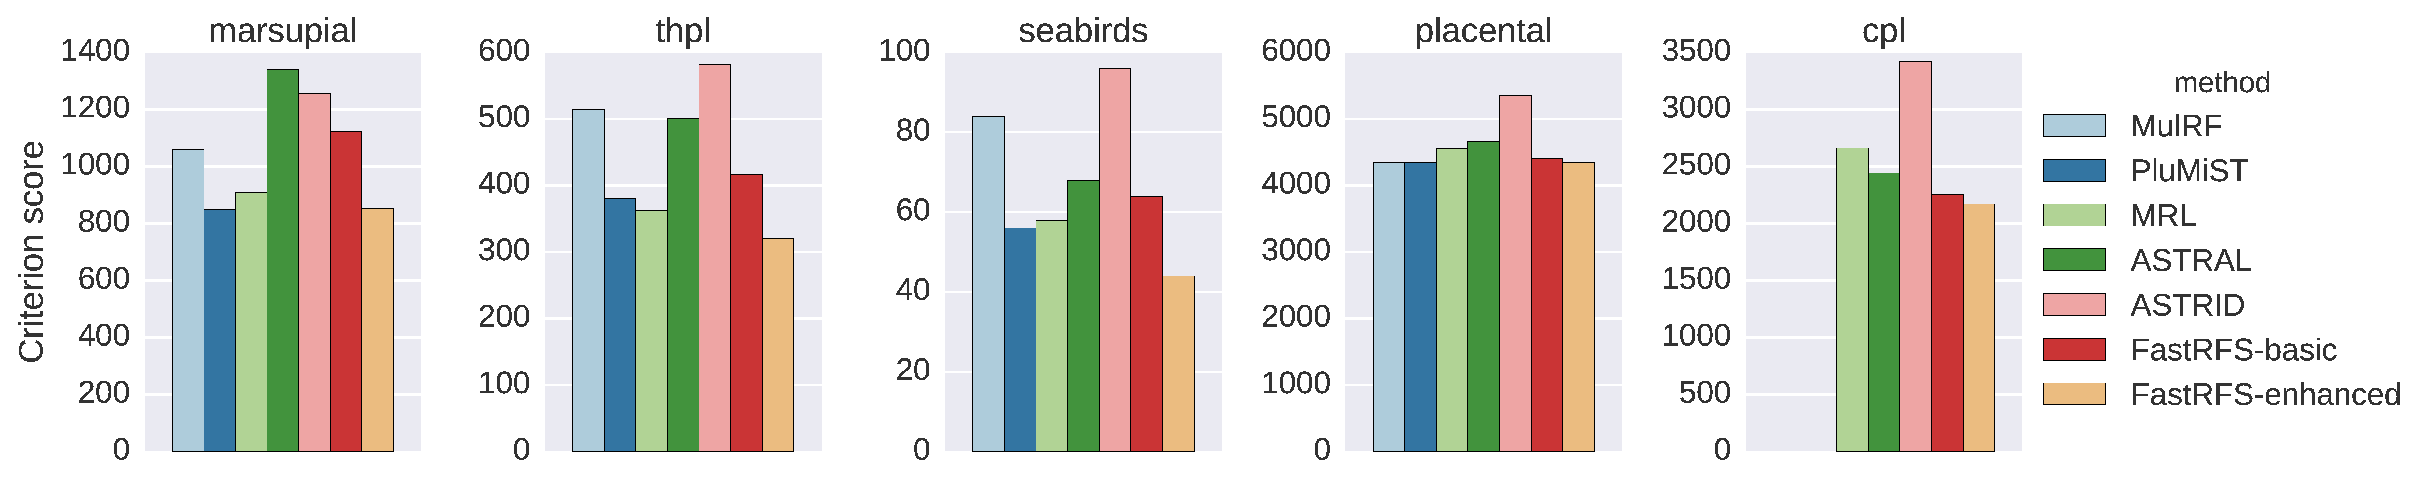
\includegraphics[width=\textwidth]{fastrfs-figs/bio-critscores.eps}
    \caption[Comparison of FastRFS and other supertree methods on five biological datasets with respect to RFS criterion score]{RFS criterion scores on biological data 
of supertree methods; lower is better.
MulRF and PluMiST could not be run on the CPL dataset due to its large size; hence
no values are shown for those methods on that dataset.
Overall, FastRFS-enhanced produces the best RFS criterion scores on these datasets.
}
    \label{fastrfs::fig:bio-critscores}
\end{figure}


 \begin{figure}
     \centering
     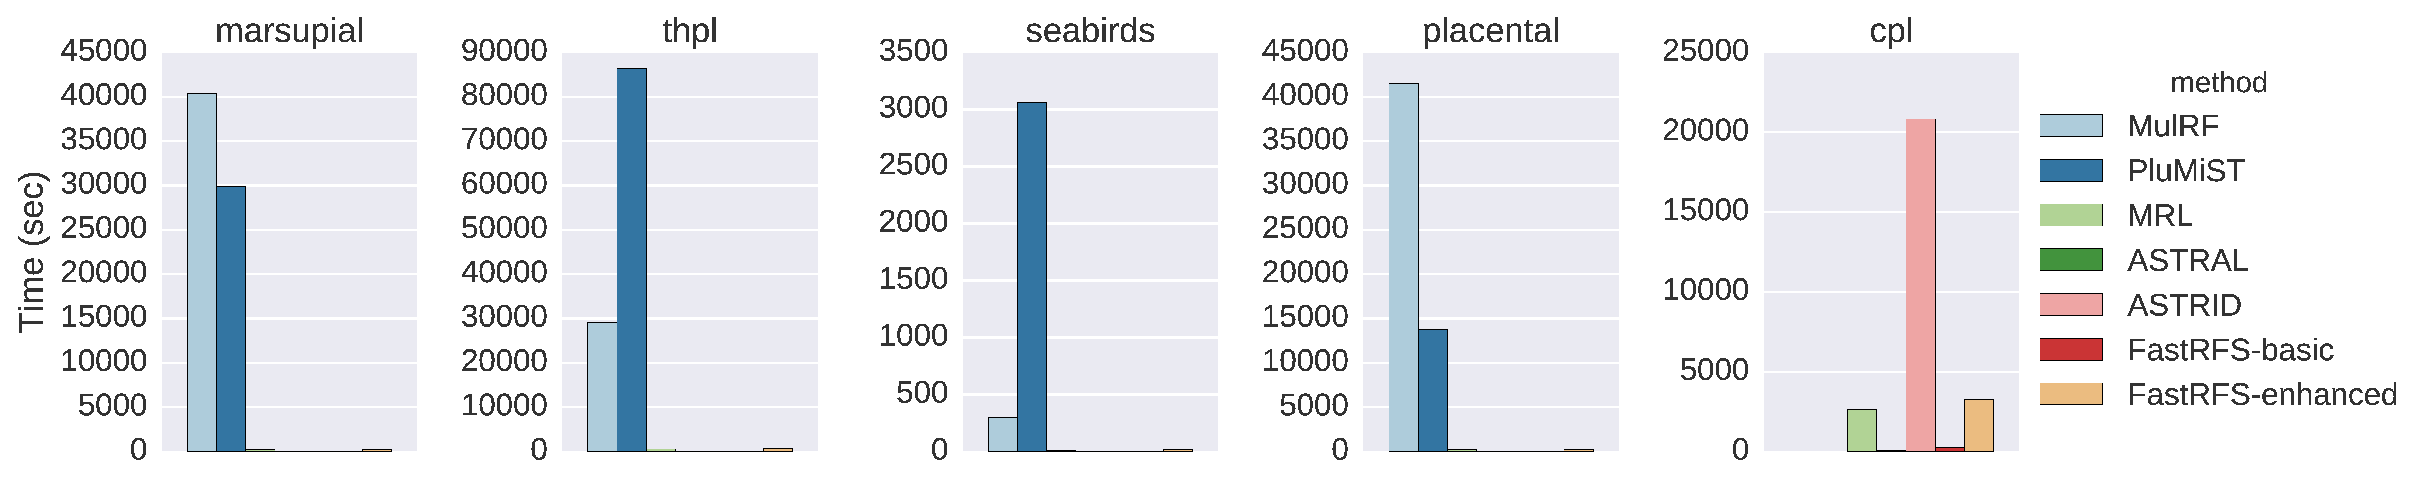
\includegraphics[width=\textwidth]{fastrfs-figs/bio-timing.eps}
     \caption[Running times of FastRFS and other supertree methods on five biological datasets]{Sequential running times (in seconds) on biological data of supertree methods. 
 MulRF and PluMiST could not be run on the CPL dataset, due to its large size; hence
 no values are shown for those methods on that dataset.
 }
     \label{fastrfs::fig:bio-timing}
 \end{figure}




\paragraph{\bf Datasets.  }
We used a collection of published simulated and biological datasets that
have been used in other studies \cite{smidgen} to evaluate supertree methods,
all of which are available online at
\url{http://www.cs.utexas.edu/users/phylo/datasets/supertrees.html}.

The simulated data, referred to as ``SMIDgen" in \cite{smidgen},
are generated
using  a taxon sampling strategy that mimics biological practice. 
These datasets have
100, 500, or 1000 taxa, with up to 25 source trees per replicate. 
Each supertree input has several ``clade-based" source trees and a ``scaffold tree", 
which are estimated using maximum likelihood heuristics on a concatenation 
of gene sequence alignments. 
Some genes are ``universal" and so are present in every species; others
evolve within the species tree under a birth-death model in which birth happens once but death (i.e., gene disappearance) can happen several times; therefore, unless the gene is born at the root of the species tree, it will be present only within a clade within the tree. Sequences then evolve down the gene trees under the GTRGAMMA model of site evolution.
The scaffold tree is based only on the universal genes, and have a random
subset of the species set; the clade-based trees are obtained by
selecting a clade in the tree and then a set of genes that covers
that clade well.
As shown in \cite{smidgen}, the density of the scaffold tree (i.e., the percentage of the full set of taxa that are in the scaffold dataset) has a large impact on the topological accuracy of the resultant estimated supertree.
 These simulated data enable us to evaluate topological accuracy as well as criterion score.
 
We include the biological datasets that were  also studied in
\cite{smidgen}:
CPL (comprehensive papilinoid
legumes) \cite{cpl},
Marsupials \cite{marsupial},
Placental Mammals \cite{placental},
Seabirds \cite{kennedy2002seabird}, 
and THPL (temperate herbaceous papilionmoid legumes) \cite{THPL}.
These range 
in size from 116 species (Placental
Mammals) to 2228 (CPL), and with
as few as 7 source trees (Seabirds) to as many as 726 (Placental Mammals).


\paragraph{\bf Methods.  }
In addition to the two FastRFS variants (basic and enhanced),
we computed supertrees using MRL, ASTRID, ASTRAL-2, MulRF, and PluMiST.
For 
MRL, 
we compute 
the MRP matrix using ``mrpmatrix" available at
\url{github.com/smirarab/mrpmatrix}, and we
use
RAxML \cite{RAxML} version 8.2.4
under the BINGAMMA model  with seed 12345 on the MRP matrix.
We ran 
MulRF version 1.2 \cite{mulrf} and
PluMiST version 1.1 \cite{plumist}.
We ran PluMiST in default mode, and we ran
MulRF ten times, and report results for the 
tree with the best criterion score.
We ran
ASTRAL-2 version 4.7.12  \cite{ASTRAL2} (henceforth
referred to as ASTRAL)
and
ASTRID version 1.1 \cite{ASTRID}, both in default mode.
Each of these methods produces fully resolved
unrooted trees.  


ASTRAL produces a supertree  that minimizes the total quartet distance
to the input source trees (equivalently, it produces a supertree that
maximizes the total quartet tree support) subject to a constrained
set $X$ of bipartitions that it computes from the input source
trees.

We tested an enhanced version of
ASTRAL (analogous to FastRFS-enhanced), in which 
we added the bipartitions from MRL and ASTRID 
to the set $X$; this enables a direct comparison of
FastRFS-enhanced and ASTRAL-enhanced. Although
FastRFS-enhanced is guaranteed to find RFS criterion scores
that are at least as good as
ASTRAL-enhanced, the comparison with respect to tree topology accuracy
makes it possible to evaluate the two optimization
criteria (minimize quartet distance or
minimize Robinson-Foulds distance) and their impact on topological accuracy.
Finally, we tested the impact of adding the bipartitions
from just one tree (MRL or ASTRID) to
the set $X$ on FastRFS, to determine the relative impact
of each additional tree.


\paragraph{\bf Measurements. }
We can use the simulated data to explore performance with respect to
criterion scores as well as tree estimation error. 
However, 
since there is no known true
supertree for the biological datasets, we use the biological 
datasets to explore performance only with respect to criterion scores.

For tree estimation error (explored only on the simulated
datasets), we
report the normalized bipartition distance (also
called the Robinson-Foulds error rate) between the
estimated and true trees.
The
Robinson-Foulds  (RF) error rate is
 $\frac{RF(T,T')}{2n-6}$, where $RF(T,T')$ is the RF distance between the true tree $T$ and the estimated tree $T'$, and $n$ is the number of leaves in $T$). 
Hence, the RF error rate is  between $0$ and $1$, and is equal to $0$ if and only if the two trees are identical. 

We also report the Robinson-Foulds Supertree criterion
score (i.e., the total Robinson-Foulds distance between the
estimated supertree
and the input source trees) for all datasets;
this value is bounded from
above by $(2n-6)k$, where $n$ is the total number of species and $k$ is the total number of source trees.

Although the criterion scores and tree error metrics both refer
to the Robinson-Foulds distance, the criterion score is based
on the RF distance to the input source trees, and the
tree error metric refers to the RF distance to the model  tree, which is unknown.
Hence these are two different ways of evaluating  methods.


Most of the methods are sequential codes; however, FastRFS is
parallelized to run on 8 cores and we run MulRF 10 times in parallel
and take the best tree.  We report wall clock running times for all
codes; except when the differences are large, comparisons between
running times are not reliable. Running times for FastRFS-enhanced
include the time to compute the MRL tree
and the ASTRID distance matrix, and, if the 
distance matrix has no missing data,   the time to run
FastME on the distance matrix (i.e., to fully compute the
ASTRID tree).

\paragraph{\bf Experiments.  }
We performed  experiments to evaluate the 
different supertree methods with respect to  
Robinson-Foulds criterion score,  topological accuracy of the supertree, and  
running time. 

\begin{table*}
\centering
\small
\begin{tabular}{|r|rrrrrrrrrrrr|}
\hline
Method&100 & 100 & 100 & 100 & 500 & 500 & 500 & 500 & 1000 & 1000 & 1000 &
1000\\
Scaffold \% &20 & 50 & 75 & 100 & 20 & 50 & 75 & 100 & 20 & 50 & 75 & 100\\
\# Replicates & 9 & 10 & 10 & 10 & 8 & 10 & 10 & 10 & 10 & 10 & 10 & 10 \\
\hline
\hline
ASTRAL& $\mathbf{11.7}$&$14.0$& $11.6$& $10.0$& $15.3$& $14.8$& $12.7$& $11.2$& $16.9$& $15.7$& $13.6$& $11.6$\\
ASTRAL-enh&$11.8$& $\mathbf{13.1}$&$11.5$& $10.0$& $14.8$&$14.1$& $12.6$& $11.2$& $\mathbf{16.3}$&$\mathbf{15.1}$&$13.5$&$11.6$\\
ASTRID& $15.8$& $18.7$& $17.1$&$9.6$&$26.0$& $50.1$& $45.4$&$\mathbf{10.5}$&$35.6$& $58.1$& $52.0$& $\mathbf{11.2}$\\
MRL&$13.6$& $13.6$& $11.2$& $10.8$& $15.4$& $14.3$& $12.1$& $11.2$& $17.4$&$\mathbf{15.1}$&$13.5$& $12.2$\\
MulRF&$22.1$& $26.0$& $15.3$& $9.3$&$46.9$& $40.3$& $27.4$& $12.6$& $-$&$-$&$-$&$-$\\
PluMiST&$25.9$& $16.6$& $11.5$& $9.3$&$35.4$& $29.5$& $22.4$& $10.9$&$-$&$-$&$-$&$-$\\
\hline
FastRFS-basic&$13.5$& $14.3$& $\mathbf{10.5}$&$\mathbf{9.1}$& $14.5$&$14.3$& $12.4$& $11.1$& $17.3$& $15.6$& $13.5$& $12.0$\\
FastRFS-enh&$13.5$& $13.4$& $10.6$& $9.3$&$\mathbf{14.3}$&$\mathbf{13.9}$&$\mathbf{12.0}$&$10.8$& $16.7$&$\mathbf{15.1}$&$\mathbf{13.4}$&$11.8$\\
\hline
\end{tabular}
  \caption[Supertree estimation error on simulated datasets for FastRFS and other methods]{Supertree topology estimation error on simulated datasets,
 measured using the Robinson-Foulds error rate, expressed
as a percentage.
The best result for each model condition is boldfaced. No results are shown
for PluMiST or MulRF on the 1000-taxon simulated datasets due to
running time limitations for these methods.
Results are averaged over the completed replicates. }
  \label{fastrfs::table:exp1-topo}
\end{table*}




\section{Results and Discussion}
\label{fastrfs::sec:results}

\paragraph{Impact of the constraint set on criterion scores. }
Our initial experiment evaluated the impact on the
criterion scores found by FastRFS of
adding bipartitions from the MRL tree and/or the ASTRID tree to the constraint
set.
In general, FastRFS with the MRL tree alone added
was nearly as good as FastRFS-enhanced (i.e.,  with both 
ASTRID and MRL trees added), and FastRFS with MRL found substantially
better criterion scores than
FastRFS with just the ASTRID tree added.
Nevertheless, since adding
the ASTRID tree did help occasionally, and since ASTRID is so quick to
run when the distance matrix is complete, we continued using it for
FastRFS-enhanced.
See Figures \ref{fig:fastrfs-sup::sim-fastrfs-comp} and \ref{fig:fastrfs-sup::bio-fastrfs-comp} for these results.


\paragraph{Criterion scores for the simulated datasets. }

By design, FastRFS-enhanced will always find criterion scores
that are at least as good as those found
by ASTRAL-enhanced, FastRFS-basic, ASTRAL, and MRL.
Hence, the only methods that could possibly find
better scores than FastRFS-enhanced are PluMiST, MulRF,
and ASTRID. 
We show the Robinson-Foulds Supertree criterion scores
in Table \ref{fastrfs::table:simulated-critscores}; note that
lower is better.
PluMiST failed to complete
on three datasets (one replicate  in the 
100-taxon and two replicates in the 500-taxon
datasets, each with 20\%-scaffolds); we report
results only on the remaining datasets. 
Both PluMiST and MulRF had very large
running times on the 500-taxon datasets; therefore, 
we did not
attempt to run them on the 1000-taxon datasets.
All other methods succeeded in completing on all
datasets we examined.

FastRFS-enhanced found the 
best (lowest) Robinson-Foulds Supertree
(RFS)
criterion scores of all methods for
all datasets; FastRFS-basic also found
these best scores for three of the four 100-taxon
model conditions, but otherwise found higher scores.
PluMiST found better RFS 
criterion scores than MulRF in 7 of the 8
model conditions, and  matched in 1 condition.
ASTRID had the worst performance of all methods,
with much larger criterion scores on all
the sparse scaffold model conditions.
These are the same conditions in which 
the internode distance matrix has missing entries, 
suggesting that
the reduced accuracy is largely due to the missing data in
the distance matrix.

Certain additional trends are worth noting.
First, although PluMiST did well on the 100-taxon
datasets, it was not so competitive with FastRFS-enhanced
or even FastRFS-basic on the 500-taxon datasets, suggesting
that 
the number of taxa may impact the ability of
PluMiST to find trees with good criterion scores.
ASTRAL-enhanced matched or improved on the
RFS criterion scores compared
to ASTRAL; this is interesting because it
does not follow from the algorithm design
(the two methods seek the tree that minimizes
the quartet distance, not the RFS criterion).
MRL, although never coming in first, often
had very good results, coming just behind
FastRFS-basic for overall performance. 








\paragraph{Criterion scores on biological datasets. }

We were unable to 
run PluMiST and MulRF on the CPL dataset, the largest
in our collection, due to its size: at 2228 species,
the running time needed for these two methods is
excessive.
Criterion scores on the biological datasets follow 
very similar patterns as observed on the simulated 
datasets (Fig.~\ref{fastrfs::fig:bio-critscores}). %(Fig.  2). %\ref{fastrfs::table:bio-rfscore}), Tandy hardwired
Overall, FastRFS-enhanced had the
best criterion scores: the best on
four datasets, and close to best on the last
dataset (Marsupials).
PluMiST tied for best with FastRFS-enhanced
on two  of the four
datasets on which it can run, 
had the second best score on seabirds,
and third best on THPL.
Hence, PluMiST is in second place.
Interestingly, the dataset on which PluMiST was
not able to find one of the top two scores
was the second largest dataset, with more
than 500 species.
Thus, just as we 
saw on the simulated datasets, the number of species seems to impact
the relative performance of PluMiST in comparison
to other methods.

The next two best methods are MRL and FastRFS-basic,
which had close performance, but MRL was
slightly better.
ASTRAL and MulRF are next, again with
mixed performance (MulRF was better
on two datasets and ASTRAL was better on the other
two). Finally, ASTRID had the worst
performance of all methods - coming in 
dead last on four of the five datasets.
It is worth noting that all but two of
the datasets produced distance matrices
with missing entries, and ASTRID did better
than ASTRAL on one 
of the two datasets (marsupial)
that produced a complete distance matrix.








\paragraph{Topological accuracy.  }
Since the true supertree is not known for the biological datasets, 
we evaluate topological accuracy only on the simulated datasets
red
(Table 2).
All methods improved in accuracy with the increase
in the scaffold density, so that error rates were
generally highest for 20\%-scaffolds and lowest
for 100\%-scaffolds.
The differences between methods on the 100\%-scaffolds
were generally small, but there were large differences
under the other conditions.
ASTRID had very 
poor accuracy except for those with
100\%-scaffolds, and MulRF and PluMiST also
had poor accuracy with the lower density scaffolds.

The remaining methods (MRL, the two ASTRAL versions, and the
two FastRFS versions)
were fairly close in accuracy.
However, MRL was never more
accurate than FastRFS-enhanced, and was only the top
performing method for one model condition 
(where
it tied with FastRFS-enhanced).
ASTRAL-enhanced was more accurate than ASTRAL on 8 conditions,
tied on 1 condition, and less accurate on 3 conditions.
FastRFS-enhanced was more accurate
than FastRFS-basic on 9 model conditions,
tied on 1 condition, and worse on 2 conditions.
FastRFS-enhanced was more accurate than
ASTRAL-enhanced on 8 
of the 12 model conditions, tied on
1 condition, and worse on 3 conditions.

FastRFS-enhanced was the
top performing method on 5 of the 
12
model conditions; the next
best performing method
was ASTRAL-enhanced, which was the top
performing method in 3 of the 12 model conditions.
Thus, overall FastRFS-enhanced provided
the best accuracy of the tested supertree methods.
These results, and especially the
pairwise comparisons,  suggest that
optimizing the Robinson-Foulds Supertree
criterion (minimize RF distance) is better than
optimizing the ASTRAL criterion (minimize
quartet distance) for supertree estimation, and
that adding bipartitions from MRL (and 
from ASTRID if its internode distance matrix
is complete) also tends to improve accuracy.

\paragraph{Running time. } 





Figure \ref{fastrfs::fig:bio-timing} 
shows running times on the biological datasets.
MulRF and PluMiST took the most time,
 each typically requiring
hours where FastRFS-basic, MRL, and ASTRAL completed in 
well under a minute (and sometimes in just a few seconds).
MRL and FastRFS-enhanced were the next most computationally 
intensive, but were
sometimes
fast, and finally 
ASTRAL, ASTRID, and FastRFS-basic were the fastest,
often completing in just seconds. 
As an example, 
the running times on the largest dataset on which
all the methods completed
(THPL, with 558 taxa) showed substantial
differences between methods:
PluMiST used 86400 seconds (i.e., 24 hours), MulRF
used 29160 seconds (i.e., 8.1 hours), 
FastRFS-enhanced used 615 seconds (just over 10 minutes), 
MRL used 575 seconds (i.e., just under 10 minutes),
and ASTRID, ASTRAL, and FastRFS-basic used under 20 seconds.

The size of $X$ impacts the running time for FastRFS, and
ranged from 1155 to 
20,233 for FastRFS-basic
and from 2485 to 48,313 for FastRFS-enhanced.
The most computationally intensive dataset
for FastRFS-enhanced is the CPL dataset, which maximizes
both the number of taxa and $|X|$; 
however, FastRFS-enhanced
completed on this dataset in 
3282 seconds (i.e., 
under an hour).
The majority of the time for FastRFS-enhanced is spent
computing the MRL tree; the other parts of the analysis 
(i.e., computing the ASTRID matrix and potentially the ASTRID
tree, computing the constraint set from ASTRAL, and running the DP
algorithm) takes very little time (typically less than a minute).


ASTRID's running time was highly variable,
but the running time is high only for
large datasets with missing entries in the
distance matrix. The reason is
that when the matrix has missing entries, ASTRID must use BIONJ*
(which takes $\Theta(n^3)$ time)
instead of FastME (which takes $\Theta(n^2)$ time).
For example, ASTRID used about 6 hours
on the CPL dataset (the only biological
dataset with these missing entries), 
but completed in just seconds on all the other
datasets. %On the CPL dataset, the ASTRID distance matrix is missing
%entries, so ASTRID uses BIONJ*, which takes $\Theta(n^3)$ time,
%instead of FastME, which takes $\Theta(n^2)$ time. 
%This is extremely
%time consuming on datasets with many taxa, like the CPL dataset, which
%has 2228 taxa.

















\section{Conclusions}


Supertree estimation is a basic bioinformatics challenge that 
is necessary for the construction of large phylogenies as well 
as for enabling statistical phylogeny estimation methods to be applied to large datasets. 
While many methods have been developed to compute supertrees, very few have
been able to provide good accuracy on datasets with many hundreds or thousands
of species.

The FastRFS methods presented
here (i.e., the basic and enhanced versions) are fast and effective techniques 
to find solutions 
to the  NP-hard Robinson-Foulds Supertree (RFS) problem.
FastRFS-enhanced in particular nearly always finds better
solutions than PluMiST and MulRF, the leading
methods for RFS,
and does so 
 in much less time.
FastRFS relies upon a dynamic programming algorithm to find an 
exact solution to its optimization problem within a constrained search space,
a strategy introduced in 
\cite{hallett2000new}
and that  is
quite different from
the heuristic search
techniques used by most phylogeny estimation methods. 
Thus, while  FastRFS, PluMiST, and MulRF all seek to optimize the same criterion, 
FastRFS is guaranteed to find an optimal solution within its constraint space but cannot return any tree that is not within the constraint space, while PluMist and MulRF are not guaranteed to find an optimal solution within any search subspace but have access to the entire treespace. 
Thus, our study suggests that
  exactly solving
an optimization problem within a constrained search space
may be a better approach than being able to search a larger space,
as long as the constrained space is selected carefully.
However, our study also shows that expanding the constraint
set beyond the input set of source trees can be highly beneficial
in terms of finding good solutions to NP-hard optimization
problems.

FastRFS-enhanced also tends to find more accurate
tree topologies than the other supertree methods
we explored. 
The improvement in topological accuracy
suggests that 
the Robinson-Foulds Supertree problem is
a good approach to supertree estimation.
The explanation for this
is likely to be the 
close relationship between the Robinson-Foulds
Supertree problem and 
the Maximum Likelihood Supertree problem
\cite{BryantSteel2009}, which
models source tree discord based on the topological distance
to the true supertree
\cite{ml-supertree}.
Thus, although a Robinson-Foulds
Supertree is not guaranteed to be identical
to a Maximum Likelihood Supertree,
good solutions to one problem are likely to be good
solutions to the other \cite{BryantSteel2009}.
Hence, 
FastRFS 
may be a good heuristic for the Maximum 
Likelihood Supertree problem,
and this may explain its good accuracy.    

There are many directions for future work.
For example, since FastRFS by design can only
search 
within the space defined by its constraint set,
finding better constraint sets may provide additional
improvements. Alternatively, FastRFS-enhanced
may provide a good starting tree
for PluMiST and MulRF, which are able to search
an unconstrained search space.
In addition, FastRFS-enhanced may be a good
initial tree for 
Bayesian supertree methods \cite{Akanni-HGT,Akanni-Bayesian} or 
heuristic searches for Maximum Likelihood Supertrees
 \cite{Akanni-MLsupertree}.
Also, like most
supertree methods, FastRFS currently only works with 
inputs where each source
tree has at most one copy of each leaf;
methods like MulRF are designed to handle inputs of  source trees
that represent gene trees, and so can
have multiple copies of each species (arising from duplication-loss
scenarios).
We will modify  FastRFS to be able to work with
such source tree inputs.

